\begin{figure}[!ht]
  \centering
    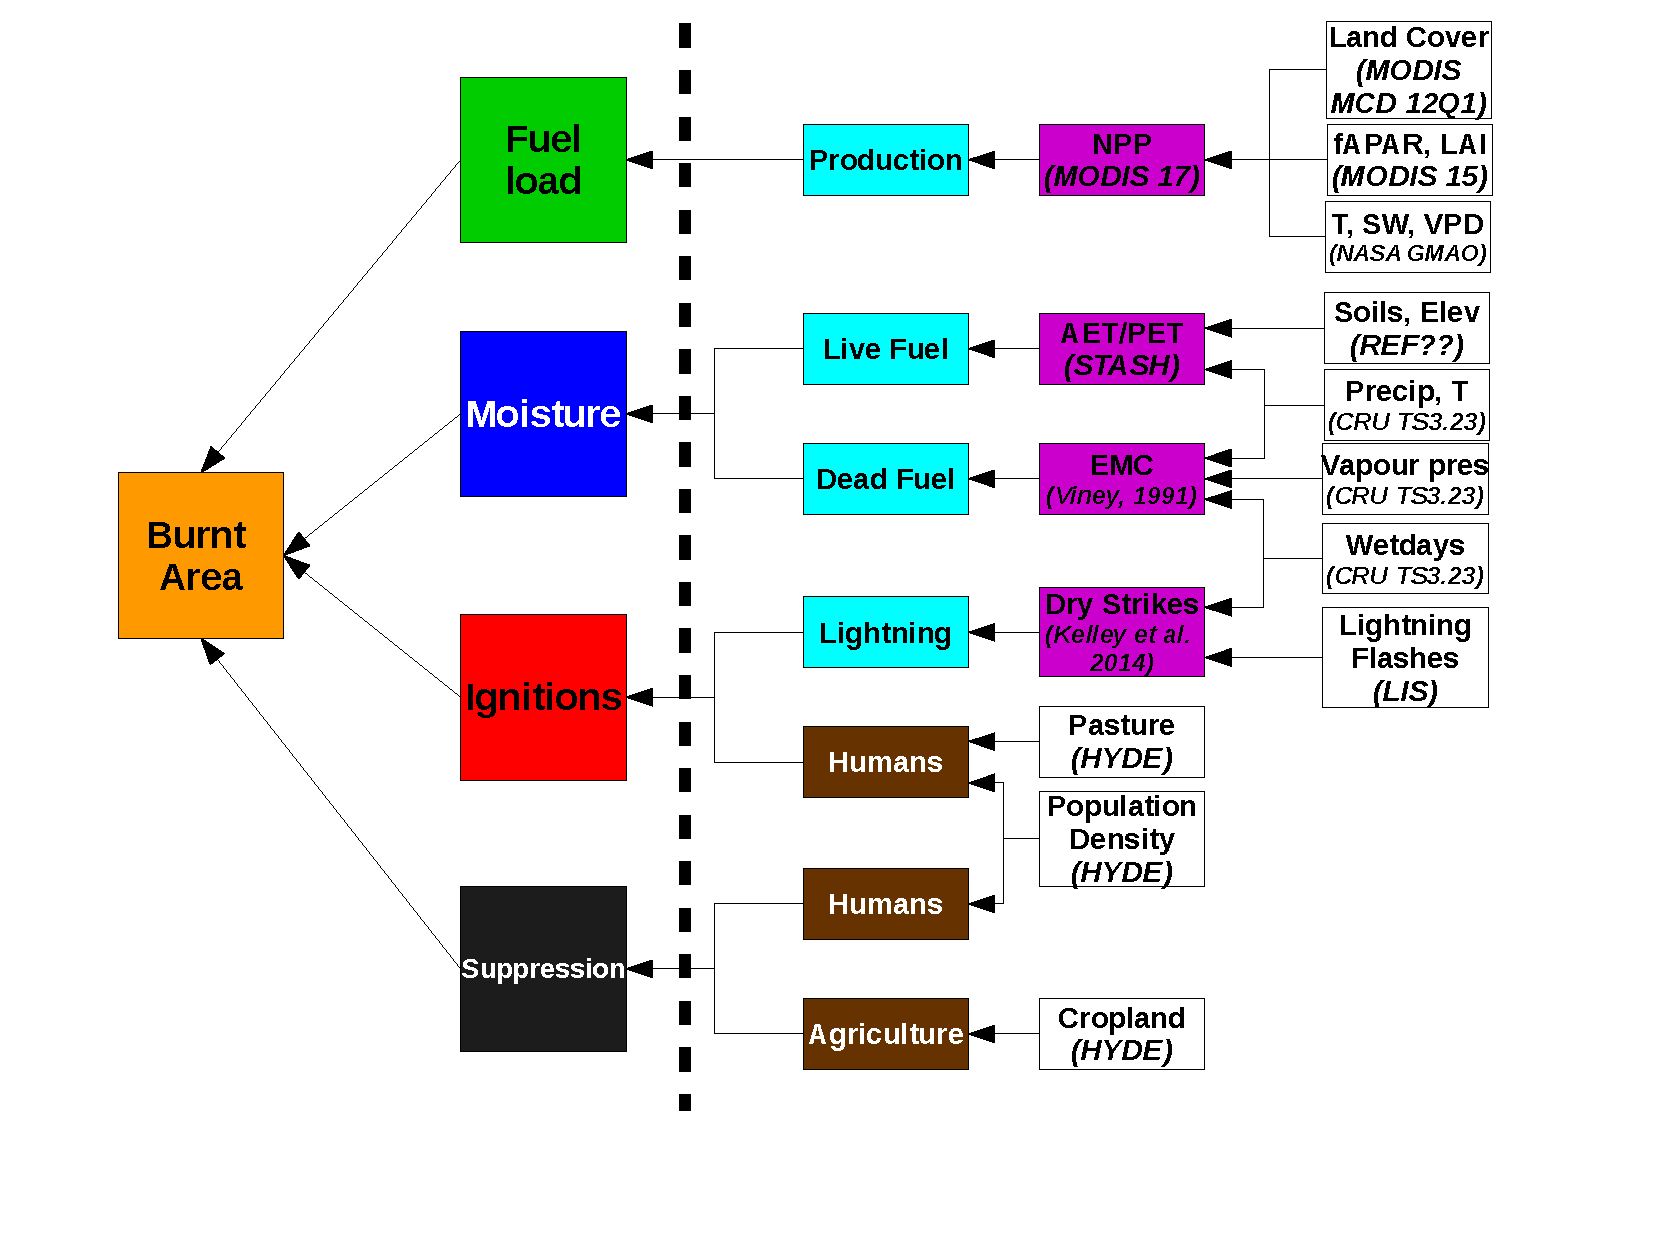
\includegraphics[width=0.67\textwidth]{Model_schematic.pdf}
  \caption{Model description.}
\end{figure}


\section{Methods}
The framework calculates burnt area based on the maximum allowed burnt area from limitations imposed by four controls: fuel, moisture, ignition, and anthropagenic supression. These controls are described from remote sensed and meteorological observations and parameters relating controls to fire are optimized against Global Fire Emissions Database (GFED4s) burnt area observations \citep{Giglio2013}.
The framework could probably be used on a range of temporal and spatial resolutions
\hlb{(scale dependancy might be something to test in the future?)}.
Here, burnt area is calculated monthly on a 0.5$^{\circ}$ CRUTS3.22 grid \citep{harris2014cru}, between Jan 2000 and Dec 2010 (the period of data overlap).

%%%%%%%%%%%%%%%%%%%%%%%%%%%%%%%%%%%%%%%%%%%%%%%%%%%%%%%%%%%%%%%%%%%%%%%%%%%%%%%%%%%%%%%%%
%% Overview                                                                            %%
%%%%%%%%%%%%%%%%%%%%%%%%%%%%%%%%%%%%%%%%%%%%%%%%%%%%%%%%%%%%%%%%%%%%%%%%%%%%%%%%%%%%%%%%%

\subsection{Overview}

The framework assumes that 100\% burnt area occurs in perfect fire conditions,  i.e. complete fuel coverage, no moisture, saturated igntions and no agricultural or urban fragmentation. This is analogous to the dry season in tropical savanna and grasslands \citep{kelley2014modelling}, particularly parts of Northern Australia \citep{murphy2013fire} and the sahel (\hlb{??Ref??}) which experiance buring each year.
Burnt area is reduced as each control becomes sub-optimal, i.e.
    fuel loads become discontinuous  (e.g. desert areas)
    or too moist (e.g. Humid evergreen forests),
    if their is lack of ignition (shown to influence inter annual variability in parts Southern Australia \cite{bradstock2010biogeographic}),
    or with increased human influance on the landscape (e.g. cropland or urban areas).
Fractional burnt area ($F$) is the product of the maximum allowed burnt area for each control ($F_i$)
\begin{equation}
    F=\Pi_{i} F_i
    \label{equ:LimFIRE}
\end{equation}

A controls maximum burnt area is related to fuel loads, moisture, ignitions and supression via the logistic function, as per \citet{bistinas2014causal} (see figure ~\ref{fig:Logistic_fun}):

\begin{equation}
    f(x) = 1 / (1 + e^{-k \cdot (x - x_0)})
    \label{equ:fx}
\end{equation}
where $k$ descibed the steepness of the curve and $x_0$ is the curves midpoint.

\begin{figure}[!ht]
  \centering
    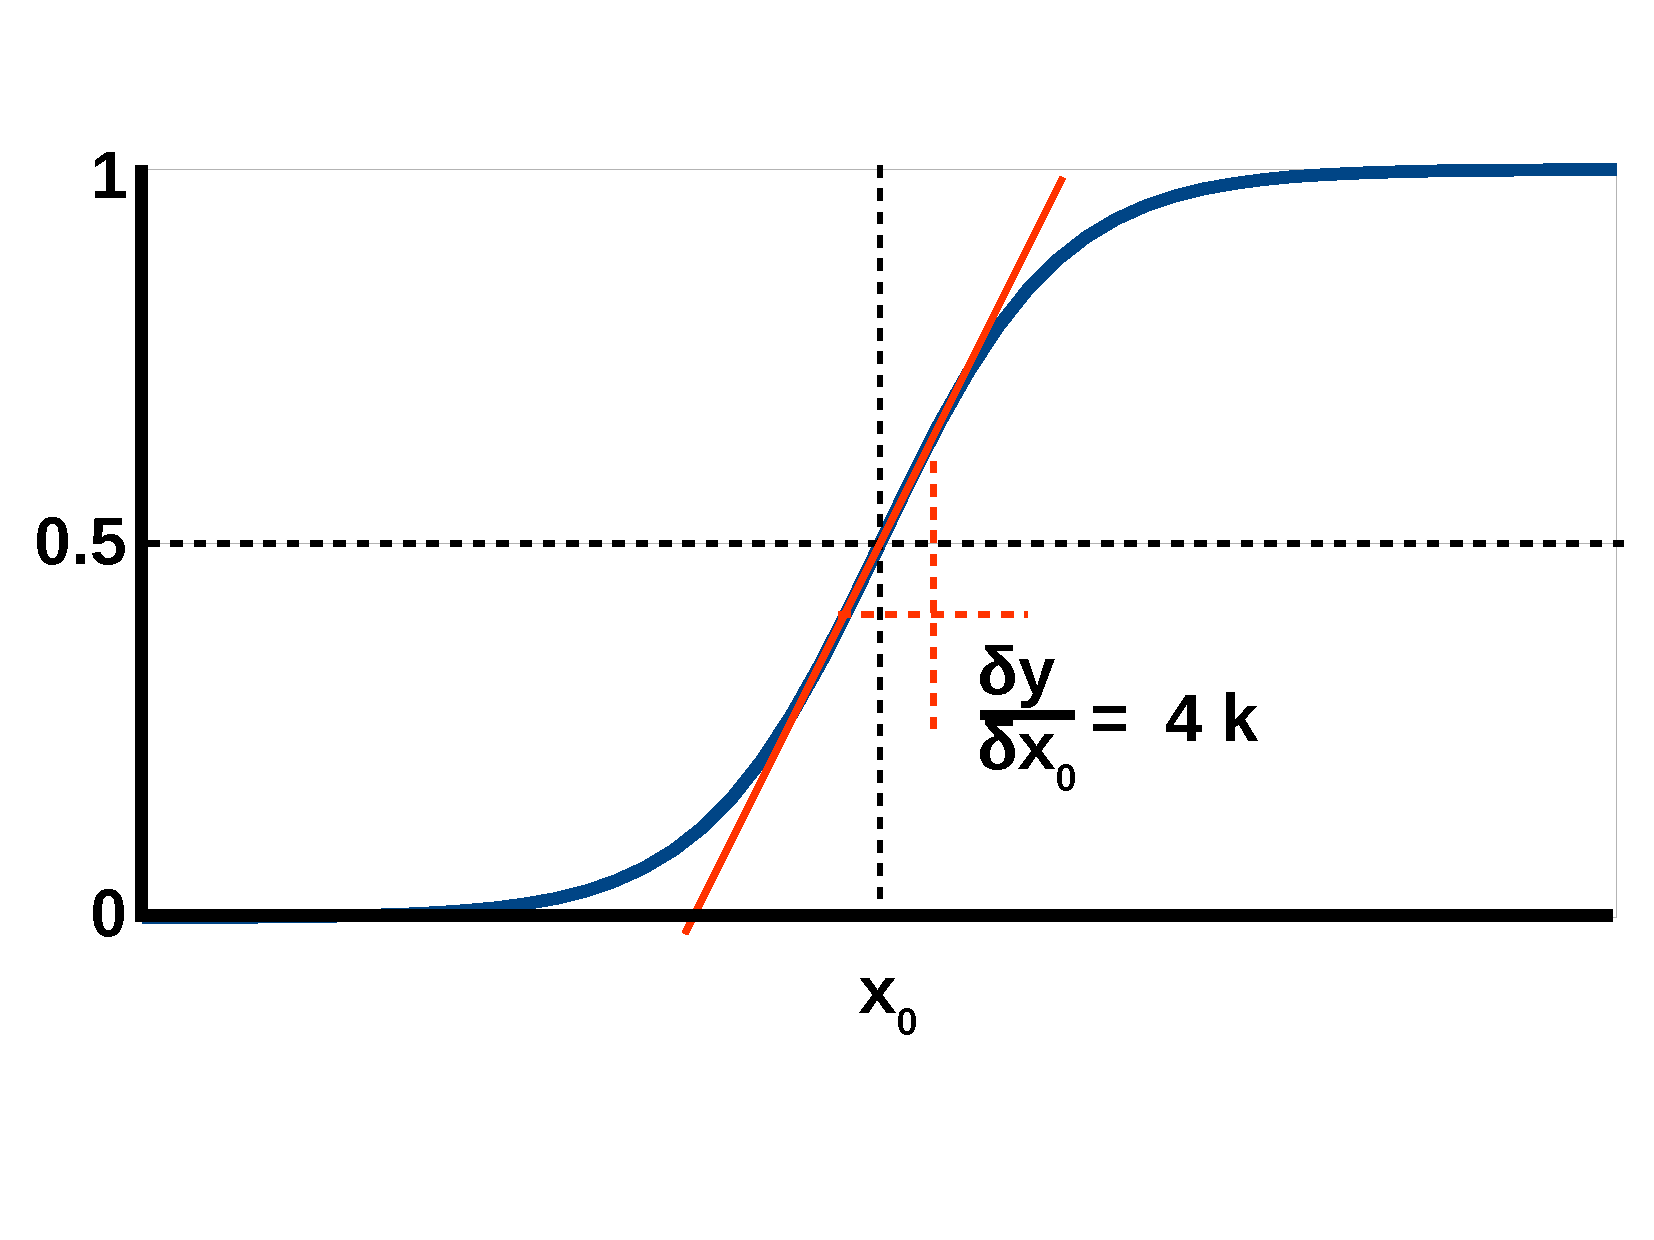
\includegraphics[width=0.67\textwidth]{Logistic_fun.pdf}
  \caption{Logistic function.}
  \label{fig:Logistic_fun}
\end{figure}

Fire increases with increasing fuel load ($F_w$) and igntions ($F_{ig}$), and decreases with moisture ($F_{\omega}$) and anthropagenic supression ($F_s$). Therefore:

\begin{equation}
    \begin{split}
        F_{w} = f(w) \\
        F_{\omega} = 1 - f(\omega) \\
        F_{ig} = f(ig) \\
        F_{s} = 1- f(s)
    \end{split}
    \label{equ:LimFIRE.x}
\end{equation}



%%%%%%%%%%%%%%%%%%%%%%%%%%%%%%%%%%%%%%%%%%%%%%%%%%%%%%%%%%%%%%%%%%%%%%%%%%%%%%%%%%%%%%%%%
%% Limitations                                                                         %%
%%%%%%%%%%%%%%%%%%%%%%%%%%%%%%%%%%%%%%%%%%%%%%%%%%%%%%%%%%%%%%%%%%%%%%%%%%%%%%%%%%%%%%%%%
\subsection{Inputs}
\begin{shaded}
\subsubsection{Fuel ($w$)}
There are two options for us to choose from:
\begin{enumerate}
    \item \textit{NPP product} as a proxy for total fuel load. Thi is the option I'm using at the moment. The product comes from Terra/MODIS Net Primary Production Yearly L4 Global 1 km MOD17A3 \citep{nasa2012terra}
    \item \textit{A measure of fractional cover} as a proxy for fuel continuity (i.e, annual mean or maximum fAPAR, as used by \citet{knorr2014impact,knorr2016climate} or MODIS fractional cover). \citet{bistinas2014causal} uses SeaWiFs fAPAR \hl{(is that right Yannis?)}, but this product finishes in 2007, so would reduce our comprison period. Other fAPAR/Fractional cover products would probably cover a larger period.
\end{enumerate}

It could be that we use the measure most apprprate for a given application. But we'd probably just use the one for the first paper?
\end{shaded}

\subsubsection{Moisture ($\omega$)}

$\omega$ represents mean fractional water content, and is split between live and dead fuel:

\begin{equation}
    \omega = (live + M \cdot dead) / (1 + M)
\end{equation}

where $M$ is an optimized parameter, representing the importance of dead fuel moisture realtive to live.

\paragraph{Live Fuel.}
The ratio of actual to potential evaporation \citep[$\alpha$][]{prentice1993simulation}, a measure of available water in relation to plant demand, is used to describe fractional water content of live fuel as per \citet{harrison2010fire, bistinas2014causal}.
$\alpha$ is calculated from CRUTS3.22 monthly mean tempuarture, cloud cover and precipitation using the STASH model \citep{sykes1996bioclimatic} r-package \citep{rstash}. \hlb{At the moment, elevation, is set to zero and field capacity to 140 - Rhys, I guess this will have to change? Any suggestions for data?}. STASH was spun up by recycling 1950 climate data for 40 years, and then run from 1950 to 2010. Simulated $\alpha$ from 2000-2010 used for the rest of the analysis.

\paragraph{Dead Fuel} moisture is represented by a simple equilibrium moisture content ($m_{mq}$) calculation from \citep{viney1991review} which combines daily precipitaion ($Pr$) and atmopheric drying potential via temprature ($T$) and relative humidity ($H_r$):

\begin{equation}
     m_{mq, daily}=
        \begin{cases}
            10 - (T - H_r) / 4 ,& \text{if } Pr\leq 3 \text{mm}\\
            100,              & \text{otherwise}
        \end{cases}
\end{equation}

On a monthly timestep, this simplifies to:

\begin{equation}
     m_{mq}=
        (10 - (T - H_r) / 4) \cdot (1 - WD)
        + 100 \cdot WD
\end{equation}
where WD is the monthly fraction of wet days from CRU TS3.22, where a wetday is defined as a day where $Pr > 3mm$. $H_r$ was calculated as the ratio of actual to saturated vapour pressure \hlb{ref??}:

\begin{equation}
    H_r = 100 \cdot AVP / SVP
\end{equation}

monthly $AVP$ is from CRUTS.22. $SVP$ was calculated from mean monthly tempuarture as per \citet{walter2000asce}

\begin{equation}
    SVP = 6.11 \cdot 10^{\frac{7.5 \cdot T}{237.5 + T}}
\end{equation}

\subsubsection{Igntions ($ig$)}

Igntions combines sources from lightning ($L_{ig}$), pasture and local population.

\begin{equation}
    ig = L_{ig} + P \cdot Pasture + D \cdot Population\text{ }Density
\end{equation}
where P and D are opimized paramters.

\begin{shaded}
    We could also add background igntions:

    \begin{equation}
        ig = 1 + N \cdot L_{ig} + P \cdot Pasture + D \cdot Population\text{ }Density
    \end{equation}
    where N, P and D are opimized paramters describing the contribution of their respective ignition source relative to background igntions.
\end{shaded}

\paragraph{Lightning}
is calculated from
from the Lightning Imaging Sensor flash count climateology (LIS \cite{christian1999lightning}, http://grip.nsstc.nasa.gov/). \hlb{Are there other products that could be used instead?}
This contains both cloud-to-ground (avavailbe for igntions) and inter-cload (not available for ignitions) strikes.
CG lighting is calculated using \citet{kelley2014improved}:

\begin{equation}
    CG = L * min(1, 0.0408 \cdot FL^{-0.4180}
\end{equation}

\begin{shaded}
\citet{kelley2014improved} also extracted dry-only lighting as available igntion sources. I'm implementing this as the moment, but I'm not to sure if I should:

\begin{equation}
    L_{ig} = 0.8533 \cdot CG \cdot e^{-2.835 \cdot WD}
\end{equation}
\end{shaded}

\paragraph{Pasture and population density}
\label{Pasture}
are taken from the HYDE dataset \citep{klein2007mapping}, and are interpolated from a decadle to a monthly timestep.

\subsubsection{Supression ($s$)}

Supression combines urban and cropland area and population desnity

\begin{equation}
    s = urban + C \cdot Crop + H \cdot Population\text{ }Density
    \label{equ:Supression}
\end{equation}

where $C$ and $H$ are optimized parameters.

\textbf{Urban} and \textbf{cropland} areas are taken from HYDE and processed as per pasture and population desnity (section ~\ref{Pasture})


%%%%%%%%%%%%%%%%%%%%%%%%%%%%%%%%%%%%%%%%%%%%%%%%%%%%%%%%%%%%%%%%%%%%%%%%%%%%%%%%%%%%%%%%%
%% Optimization                                                                        %%
%%%%%%%%%%%%%%%%%%%%%%%%%%%%%%%%%%%%%%%%%%%%%%%%%%%%%%%%%%%%%%%%%%%%%%%%%%%%%%%%%%%%%%%%%
\subsection{Optimization}

\begin{shaded}
The framework is optimized against GFED4s observations \citep{Giglio2013}  using normalised least square r-package \citep{rstats}. GFED4s was regridded from 0.25 to a 0.5$^{\circ}$ resolution using ``resample'' in the raster r-package \citep{rraster}. This is likley to change though, so I wont descibe it any more for the moment.
\end{shaded}

Optimization is performed on equation ~\ref{equ:LimFIRE} to ~\ref{equ:Supression}. Each limitation optimizes two parameters associated with it's maximum expected burnt area (equations ~\ref{equ:fx} and ~\ref{equ:LimFIRE.x}, see figure ~\ref{fig:Logistic_fun}).
Paramters relating different fuel moisture, ignition and supressions sources are also optimzed (see table ~\ref{tab:optimize})

\begin{table}[]
\centering
\caption{Optimized paramters obviosuly, to be filled in.}
\label{tab:optimize}
\begin{tabular}{llll}
\hline
\multicolumn{2}{c}{\textbf{Parameter}} & \multicolumn{1}{c}{\textbf{Bound}} & \multicolumn{1}{c}{\textbf{Value}} \\ \hline
\multirow{2}{*}{Fuel}             & $k_{w}$         &                                    &                                    \\
                                  & $x_{0,w}$       &                                    &                                    \\ \hline
\multirow{3}{*}{Moisture}         & $k_{\omega}$    &                                    &                                    \\
                                  & $x_{0, \omega}$ &                                    &                                    \\
                                  & $M$             &                                    &                                    \\ \hline
\multirow{4}{*}{Igntions}         & $k_{ig}$        &                                    &                                    \\
                                  & $x_{0, ig}$     &                                    &                                    \\
                                  & $P$             &                                    &                                    \\
                                  & $D$             &                                    &                                    \\ \hline
\multirow{4}{*}{Human Supression} & $k_{s}$         &                                    &                                    \\
                                  & $x_{0, s}$      &                                    &                                    \\
                                  & $C$             &                                    &                                    \\
                                  & $H$             &                                    &                                    \\ \hline
\end{tabular}
\end{table}
%%%%%%%%%%%%%%%%%%%%%%%%%%%%%%%%%%%%%%%%%%%%%%%%%%%%%%%%%%%%%%%%%%%%%%%%%%%%%%%%%%%%%%%%%
%% Benchmarking                                                                        %%
%%%%%%%%%%%%%%%%%%%%%%%%%%%%%%%%%%%%%%%%%%%%%%%%%%%%%%%%%%%%%%%%%%%%%%%%%%%%%%%%%%%%%%%%%
\subsection{Benchmarking}
\begin{shaded}
To assess performance of reconstructed burnt area, we'll probably use NME for annual average, seasonal and inter-annual comparisons \citep{kelley2013comprehensive} as reccomended by fireMIP \citet{gmd-2016-237, hantson2016status}, and maybe McFaddens $R^{2}$ as per \citep{bistinas2014causal}. Annual average NME comparison comes out at 0.46, which is better then benchmarking null models descibed in \citet{kelley2013comprehensive}, and outperforms coupled vegetation-fire models contributing to fireMIP \citep{hantson2016status}, although this is to be expected as the framework is driven by and optimized to observations \citep{kelley2013comprehensive}.

Yannis/Rhys - any thoughts on this?
\end{shaded}
%%%%%%%%%%%%%%%%%%%%%%%%%%%%%%%%%%%%%%%%%%%%%%%%%%%%%%%%%%%%%%%%%%%%%%%%%%%%%%%%%%%%%%%%%
%% Analysis                                                                            %%
%%%%%%%%%%%%%%%%%%%%%%%%%%%%%%%%%%%%%%%%%%%%%%%%%%%%%%%%%%%%%%%%%%%%%%%%%%%%%%%%%%%%%%%%%
\subsection{Analysis}


\subsubsection{Limitation}

The relative importance of each controls was assessed as:

\begin{equation}
    \bar{L_{i, X}} = \frac{L_{i, X}}{\sum_{j} L_{j, X}}
\end{equation}
where $L_{i, X} = 1 - F_{i,X}$ is the individual contribution of each control $i$ for conditions $X$.

\subsubsection{Sensitivity}



\begin{shaded}
    There's two ways I can think of that we could assess sensitivity to each control. We could compare the gradient of each control around the cells current conditions. Alterntaive, we could calculate the required change in each control to induce a ``significant'' change in fire regime. The first would be a nice way of classificying different locations, along the same way as limitarions (i.e, Australian Tropical Savanna is xx \% senstiave to changes in fuel load, and yy \% to moisture). The second would be harder to normalise across controls, but might be easier to relate to actual changes in climate (i.e, xx $^{\circ}$ increase in tempurature would increase fire to expected levels for Savanna; increase in yy \% of agriuclutural land would reduce fire in non-agricultural land to that expected for forests etc)

\paragraph{options 1}

\begin{equation}
    \bar{\partial L_{i, x}} = \frac{\partial L_{i, x} \cdot \Pi_{j} L_{j, x}}{L_{i, x}}
\end{equation}

where $\partial L_{i, x}$ is the gradient of $L_{i, x}$ relative to the maximum possible gradient of $L_{i}$, occuring when $x = x_{0}$ i.e:

\begin{equation}
    \partial l_{i, x} = \frac{\partial l_{i, x} / \partial X}
                             {\partial l_{i, x_{0}} / \partial x}
\end{equation}

\paragraph{options 2}
for measuring sensitivity is to calculate the change required for a control to alter burnt area enough to induce major alterations in i.e vegetation cover.
For example, assessing amazon risk of fire-induced tipping point. Holding the contribution of ignition, fuel load and land use constant, we could calculate the change in moisture needed to increase burnt area to the level expected for Savanna (roughly 1\% in South America according to \cite{lehmann2011deciphering}).
It would be easy to work out a required change in climate variables (humidity, temperature, ET etc, or any combination of these) required to hit this 'fire tipping point'.

\end{shaded}
